\chapter{CONCEITOS E TÉCNICAS NECESSÁRIAS}

O capitulo explica termos técnicos essenciais para o melhor entendimento do trabalho.

\section{Samba}

/* Samba é um software open source e reimplementa os protocolos SMB e CIFS para prover
uma série de serviços para ambiente Windows, como servidor de arquivos e impressão e pode
ser usado em um Servidor de Domínio como um Primary Domain Controller (PDC) ou como
como um membro do domínio, e pode também ser usado como parte de um domínio Active
Directory. */

Samba é um software open source que provê serviços a clientes nos protocolos SMB e CIFS.
O samba permite a interoperabilidade entre servidores Linux/Unix e clientes baseados na
plataforma Windows.
O samba permite que um servidor linux seja apto a fornecer serviços como:
  \begin{itemize}
    \item \textbf{\#Servidor de arquivos e impressão} Utilizando o protocolo Server Message Block para possibilitar o compartilhamento de arquivos, pastas volumes e impressoras na rede.

    \item \textbf{\#Autenticação e autorização} Identifica um computador ou um usuário da rede e determina os direitos de acesso a arquivos que cada usuário possui, através de tecnologias como permissões de arquivos, diretivas de grupo e o serviço de autenticação Kerberos.

    \item \textbf{\#Resolução e busca de nomes e diretórios} Compartilha as principais informações sobre computadores e usuários da rede através do Light Directory Access Protocol (LDAP) e o Microsoft Active Directory.

    \item \textbf{\#Servidor de domínio como PDC} Funcionando como controlador de domínio ativo dentro de um domínio Windows.
  \end{itemize}

Basicamente, o Samba é um servidor e um conjunto de ferramentas que permite ocompartilhamento de arquivos e impressoras sistemas Windows e Linux. Usando o Samba emum servidor Linux, ele se comporta exatamente como um servidor Windows, podendoinclusive autenticar usuários e compartilhar impressoras. Outra característica do Samba é que ele pode atuar como um Controlador Primário de Domínio (PDC), armazenando perfis deusuários, realizar controle de acesso, sendo suas as configurações tão efetivas quanto às de umservidor Windows (FOCA, 2007).

\section{Permissões no Linux}

\section{Permissões especiais no Linux}

Existe no Linux três permissões especiais, para dar segurança ao sistema, chamadas assim por somente serem atribuídas a arquivos específicos (arquivos executáveis e diretórios). Tais permissões são fornecidas pelos bits SUID, SGID e STICKY.

  \begin{itemize}
    \item \textbf{\#SUID} O bit SUID (Set UID) é aplicável apenas a arquivos executáveis, fazendo com que estes rodem com as permissões de seu proprietário, independente de quem tenha executado-o. Pode ser útil para que usuários comuns possam executar arquivos permitidos apenas a administradores.

    \item \textbf{\#SGID} O bit SGID (Set GID) pode ser aplicado a um arquivo executável e a um diretório. No primeiro caso ele tem as mesma função do SUID, porém rodando com as permissões de um grupo de usuários. No segundo, ele força os arquivos e diretórios criados dentro do diretório pai (o que obteve a permissão) a pertencerem ao mesmo grupo, independente do grupo de quem tenha-os criado.

    \item \textbf{\#STICKY} O bit STICKY é aplicável a diretórios e faz com que a exclusão de arquivos pertencentes a estes diretórios seja apenas permitida ao dono do arquivo e ao administrador do sistema. Tem vantagem sobre a permissão “Somente Leitura” no diretório pois faz com que outros usuários possam criar e editar qualquer arquivo, impedindo-os apenas de apagá-lo.
  \end{itemize}

\section{Seções}

No Samba, as configurações de compartilhamentos, configurações de impressoras e todas as configurações gerais, são realizadas através de um unico arquivo de configuraçõa, o "/etc/samba/smb.conf". Esse arquivo para melhor organização, fica dividio em sessões, sendo a primeira sessão nomeada como [global], onde são definidas as configurações gerais do servidor. Também podem ser criadas sessões adicionais para cada compartilhamento, sendo nomeadas com o nome do mesmo. Se desejamos criar um compartilhamento com o nome "arquivo", a sessão que deve ser criada no arquivo de configuração deve ser [arquivo].

\section{Parâmetro}

\section{Variáveis}

\section{Variáveis Especiais do Samba}

\section{PDC}

Além da função de servidor de arquivos, o Samba pode ser usando também comoControlador de Domínio ou DC (Domain Controller 
), também conhecido como Controladorde Domínio Primário ou PDC (Primary Domain Controller) (MORIMOTO, 2005).

O Controlador de Domínio é responsável por fornecer autenticação para os clientes,sejam sistemas Linux ou Windows. Ou seja, apenas centraliza contas de usuários e fornecerecursos voltados para a administração de usuários, como a gestão de perfis móveis, que sãoas configurações de usuários que são lidas, independente de qual máquina o usuário utilize.Em uma rede de com pouco mais de 10 clientes a necessidade de ter um PDC é mais aparente,pois fica cada vez mais difícil de gerenciar as contas de clientes e máquinas conforme ocrescimento da rede. Com o Controlador de Domínio também é possível fornecer acesso porperfis móveis onde o usuário pode ter acesso à sua área de trabalho independente da máquina (da mesma rede) onde faz o login. Em contrapartida, bloqueando uma conta de usuário,automaticamente este estará bloqueado em todas as máquinas gerenciadas pelo Controladorde Domínio (MORIMOTO, 2005)

\section{Comandos Básicos do Samba3}

\section{SMBD}

É um daemon que permite compartilhamento de arquivos e impressoras em uma rede SMB e provê autorização e autenticação a usuários SMB. O SMBD é um dos componentes principais do Samba, e 

\section{NMBD}

É um daemon que cuida do Windows Internet Name Service (WINS) e auxilia com a navegação e resolução de nomes.

\section{NETBIOS}

NETBIOS, Networking Basic Input/Outbut System, é uma API desenvolvida em 1984 pela IBM, que fornece serviços relacionados na camada de sessão do modelo OSI, permitindo a comunicação entre computadores na rede através de um nome NETBIOS correspondente a um hostname.

\section{Domain Master}

***VERIFICAR REFERENCIA***

DOMAIN MASTER BROWSER Uma vez que o Local Master Browser é eleito no segmento de rede, uma consulta é feita ao servidor WINS para saber quem é o Domain Master Browser da rede para enviar a lista de compartilhamentos. A máquina escolhida como Local Master Browser envia pacotes para a porta UDP 138 do Domain Master e este responde pedindo a lista de todos os nomes de máquinas que o Local Master conhece e também o registra como Local Master para aquele segmento de rede.

\section{WINS}

Windows Internet Name Service (WINS) ou NetBIOS Name Service (NBNS) é um serviço do protocolo TCP/IP. Este serviço faz a resolução nomes e números IP e os armazena, disponibilizando esta informação para quem necessite usar. Cada cliente envia seu nome NetBIOS e número IP para o servidor WINS, que armazena estas informações em um banco de dados. Quando um cliente desejar se comunicar com um outro, ele envia o nome desejado ao servidor WINS. Se o nome constar na base de dados, o servidor WINS retorna ao solicitante o número IP.

\section{DNS}

DNS (Domain Name System) é uma base de dados hierárquica e distribuída, usadapara a resolução de nomes de domínios em endereços IP. É considerado como um banco dedados distribuído que converte nomes de hosts (máquinas) para endereços IP. É basicamenteum mapeamento de endereços IP e seus respectivos nomes. A utilização mais comum é nainternet. Todos os computadores da rede possuem um endereço IP. Os servidores DNSsimplesmente transformam ou resolvem esse o número em um nome. Por exemplo, oendereço www.meudominio.com.br corresponde ao IP 10.0.0.1. (SCRIMGER.R. et al, 2002)

\begin{figure}[ht]
   	\centering
    \scalebox{1}{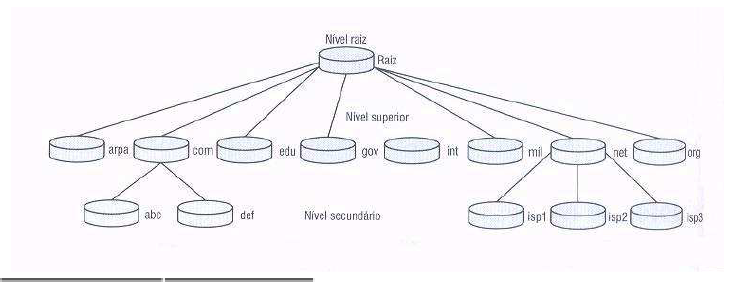
\includegraphics{figuras/dns}}
   	\caption{Estrutura hierárquica do DNS (SCRIMGER.R. et al, 2002)}
    \label{dns}
\end{figure}
figura 5 - Estrutura hierárquica do DNS (SCRIMGER.R. et al, 2002)


\section{BIND}

\section{Ldap}

O LDAP é o protocolo responsável por fornecer Serviço de Diretórios a computadores Windows de forma similar ao Active Directory da Microsoft, que é baseado no LDAP. Tais serviços incluem conexões de computadores, grupos de computadores, usuários, administração de identidades, além de possibilitar uma maneira eficiente de descrever, localizar e administrar esses recursos.

LDAP (Lightweight Directory Access Protocol) é um protocolo para acessarinformações contidas em um diretório. Por ser um protocolo cliente/servidor o LDAP permitenavegar, ler, armazenar e pesquisar informações e realizar tarefas de gerenciamento em umserviço de diretórios. O serviço de diretório é um banco de dados otimizado para leitura,navegação e pesquisas (TRIGO, 2007).

\begin{figure}[ht]
   	\centering
    \scalebox{1}{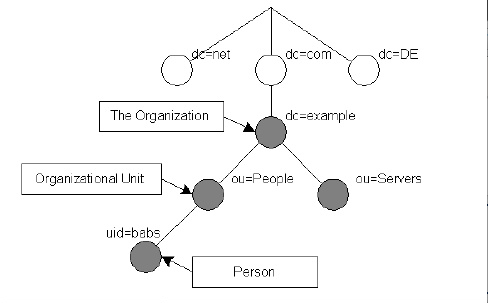
\includegraphics{figuras/ldap}}
   	\caption{Estrutura do protocolo LDAP (OPENLDAP FOUNDATION, 2003)}
    \label{ldap}
\end{figure}
figura 6 - Estrutura do protocolo LDAP (OPENLDAP FOUNDATION, 2003)

\section{Kerberos}

Kerberos é um protocolo de segurança de rede e fornece autenticação entre conputadores e usuários através de um servidor centralizado que concede autenticações criptograficas a qualquer computador utilizando o Kerberos. Esse sistema de segurança e autenticação agraga diversos benefícios como autentificação mútua, autentificação delegada, interoperabilidade e gerência simplificada e confiável. O samba pode usar o Kerberos como um mecanismo autenticação de computadores e usuários.

O Kerberos é um protocolo que prevê forte autenticação entre aplicações cliente-servidor e usa criptografia de chave simétrica no qual servidores fornecem acesso aos serviçossolicitados pelos clientes, caso provem que são eles mesmos. (FILHO. M. M. C, 2009)

O Kerberos não autentica o host no servidor, apenas a aplicação que oferece o serviço.Ele trabalha com tickets , servindo para provar a autenticidade de um usuário e garantir oacesso aos serviços e aplicações. (CONECTIVA, 2009).

Quando um usuário entra com as informações de login , considerando que seja umusuário cadastrado no KDC (é o servidor Kerberos), os dados são enviados para o servidor 25Kerberos que recebe as informações e as confere com as que estão cadastradas no banco dedados. Estas informações são criptografadas com a própria senha do usuário e enviadas devolta para ele. Este é o ticket TGT (Ticket-Grant-Ticket). Se as informações do ticket TGTpuderem ser descriptografadas, então o usuário é quem diz ser. O TGT é armazenado namáquina e, por segurança, tem um tempo de vida útil para o caso de ser interceptado na rede.(CONECTIVA, 2009)

\begin{figure}[ht]
   	\centering
    \scalebox{1}{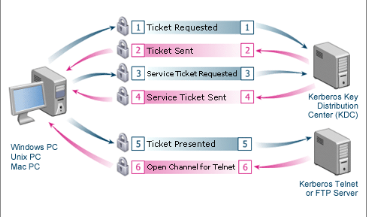
\includegraphics{figuras/kerberos}}
   	\caption{Autenticação Kerberos (CONECTIVA, 2009)}
    \label{kerberos}
\end{figure}
figura 7 - Autenticação Kerberos (CONECTIVA, 2009)

\section{NTP}

NTP (Network Time Protocol) é usado para sincronizar relógios de computadores narede local ou na internet (RNP, 2009).

\section{NTVFS}

Sistema de arquivos que armazena os atributos do NTFS

\section{GSSAPI}

A GSSAPI é uma interface que permite desenvolvedores escreverem aplicações que aproveitam mecanismos de segurança tais como Kerberos, sem ter de programar explicitamente para qualquer mecanismo, ou seja, aplicações genéricas do ponto de vista de segurança. Programas que usam GSSAPI são, deste modo, altamente portáteis, não somente de uma plataforma para outra, mas de uma configuração de segurança a outra e de um protocolo de transporte a outro. A GSSAPI fornece vários níveis de proteção de dados, consistentes com os mecanismos de segurança subjacentes.


\section{Referencias - Temporário}
SAMBA:
http://pt.wikipedia.org/wiki/Samba\_(servidor)

http://en.wikipedia.org/wiki/Samba\_(software)

http://www.samba.org/samba/docs/

http://www.samba.org/samba/what\_is\_samba.html

http://www.samba.org/samba/docs/SambaIntro.html

http://www.samba.org/cifs/docs/what\-is\-smb.html

http://www.samba.org/cifs/

Using Samba (OREILLY)

NETBIOS:

http://pt.wikipedia.org/wiki/Netbios

Using Samba (OREILLY)

SMBD: 

Using Samba (OREILLY)
http://www.samba.org/samba/docs/

NMBD:

Using Samba (OREILLY)
http://www.samba.org/samba/docs/

GSSAPI:
http://www.gta.ufrj.br/grad/10\_1/kerberos/gssapi.html

POSTFIX.ORG.BR. Disponível em: http://www.postfix.org/LDAP\_README.html\# config.Acesso em dezembro de 2009.

RNP - REDE NACIONAL DE ENSINO E PESQUISA.Apresenta descrição do protocoloNTP. Disponível em: http://www.rnp.br/ntp/. Acesso em outubro de 2009.

SAMBA.ORG-1.Samba4 / Active Directory. Disponível em:http://wiki.samba.org/index.php/Samba4/ActiveDirectory. Acesso em: dezembro de 2009

SAMBA.ORG-2.Apresenta informações sobre schemas e ldap. Disponível em:http://wiki.samba.org/index.php/Samba4/LDAP\_Backend. Acesso em dezembro de 2009.

SAMBA.ORG-3. Instalação e configuração do Samba 4. Disponível em:http://wiki.samba.org/index.php/Samba4/HOWTO\#Step\_1:\_download\_Samba4. Acessoem outubro de 
2009.

SCRIMGER.R.;LASALLE.P.;PARIHAR.M.;GUPTA.M.TCP/IP - A Bíblia. Rio de Janeiro.Campus. 2002. 642 p.

THE OPENLDAP FOUNDATION.OpenLdap 2.1 Administrator's Guide. Disponível em:http://www.bind9.net/manual/openldap/2.1/intro.html. Acesso em dezembro de 2009.

TRIGO.C.H.OpenLDAP - Uma Abordagem Integrada
. São Paulo. Novatec. 2007. 239 p.UFRJ.

Apresenta funcionamento do protocolo CIFS. Disponível em:http://www.gta.ufrj.br/grad/01\_2/samba/smbcifsinternamente.htm. Acesso em outubro de2009.

Ldap Browser. Versão 2.6. Softerra. 2004.

ALECRIN. E. Servidor Samba: o que é. Disponível em:http://www.infowester.com/linuxsamba.php. Acesso em dezembro de 2009.

CONECTIVA. Kerberos. Autenticação do Sistema. Disponível em:http://www.conectiva.com/doc/livros/online/10.0/servidor/pt\_BR/ch13s04.html. Acessoem outubro de 2009

ERICH. S. M.Autenticação Integrada Baseada em Serviço de Diretório LDAP. Apresentaestudo do protocolo LDAP. Disponível em http://www.linux.ime.usp.br/~cef/mac499-06/monografias/erich/html/ch01s05.html. Acesso em dezembro de 2009

FILHO.M.M.C. Kerberos. Apresentação do protocolo Kerberos. Disponível em:http://www.gta.ufrj.br/grad/99\_2/marcos/kerberos.htm. Acesso em julho de 2009

FOCA GNU/Linux. Samba. Disponível em: http://www.guiafoca.org/guia/avancado/ch-s-samba.htm. Acesso em novembro de 2009.

LDAP.ORG.BR Como instalar um PDC Samba+OpenLDAP. Disponível em:http://www.ldap.org.br/modules/ldap/files/files///samba+openLDAP+qmail.pdf. Acessoem setembro de 2009.

Linux Magazine. São Paulo. Linux New Media do Brasil Editora Ltda. 2009. Mensal. ISSN1806-9428.

LOSANO.M. Introdução ao Active Directory. Apresenta visão geral do Active Directory.Disponível em: http://technet.microsoft.com/pt-br/library/cc668412.aspx. Acesso emagosto de 2009.

MICROSOFT-1. Simple Network Time Protocol. Apresenta detalhes do protocolo SNTP.Disponível em: http://msdn.microsoft.com/pt-br/library/aa919019.aspx. Acesso emagosto de 2009

MICROSOFT-2. Descrição dos protocolos do Active Directory. Disponível em:http://technet.microsoft.com/pt-br/library/cc961766\%28en-us\%29.aspx. Acesso emsetembro de 2009.

MINASI. M; ANDERSON. C.;SMITH. B.M;TOOMBS.D. Dominando o Windows 2000Server. São Paulo. Pearson Education do Brasil. 2001. 1275 p.

MICROSOFT-3. Apresenta as operações mestres do Active Directory. Disponível emhttp://technet.microsoft.com/pt-br/library/cc716426.aspx. Acesso em dezembro de 2009.

MORIMOTO.C.E. Redes e Servidores Linux - Guia Prático. Porto Alegre. Sul. 2005. 302p.